\documentclass[11pt]{article}

%opening
\usepackage{caption}
\usepackage{mcexam}
\usepackage{amsmath}
\usepackage{amsfonts}
\usepackage{graphicx}
\usepackage{enumerate}
\usepackage{tikz}
\usepackage{float}
\usepgflibrary{arrows}
\usepackage{todo}
\everymath{\displaystyle}
\pagestyle{empty}
\usepackage{lastpage} % this calculates the page number of the last page
\usepackage{fancyhdr}
\pagestyle{fancy}
\lhead{\textsf{Spring 2017}}
\chead{\textsf{Math 131 -- Final Exam B}}
\rhead{\textsf{Page \thepage\ of \pageref{LastPage}}}
\cfoot{}
\rfoot{\textsf{\thepage}}

\newcommand{\series}[3]{\displaystyle \sum_{{#1}={#2}}^{#3} }
\newcommand{\limit}[2]{\displaystyle \lim_{{#1} \rightarrow {#2}} }
\newcommand{\din}[2]{\displaystyle \int_{#1}^{#2}}
\newcommand{\Int}{\displaystyle \int}
\newcommand{\Q}{\ensuremath \mathbb{Q}}
\newcommand{\R}{\ensuremath \mathbb{R}}
\newcommand{\C}{\ensuremath \mathbb{C}}
\newcommand{\Z}{\ensuremath \mathbb{Z}}
\newcommand{\N}{\ensuremath \mathbb{N}}
\newcommand{\isom}{\ensuremath \cong}
\newcommand{\inv}{\ensuremath ^{-1}}
\newcommand{\ot}{\ensuremath \otimes}
\newcommand{\op}{\ensuremath \oplus}

\Course{Math 131}{Principles of Calculus}
\Instructor{Paul Gustafson}
\TestName{Final Exam B\hfill{\bfseries\Huge GREEN}}
\Date{}
%\Section{}


\begin{document}
\Head
\begin{instructions}
\item Simplify your answers.
\item Calculators are allowed.
\item Should you have need for more space than is allocated to answer a question, use the back of the exam.
\item \textbf{Honor Code:}

\vspace{0.1in}
An Aggie does not lie, cheat, or steal or tolerate those who do.
\vspace{0.3in}

\par\noindent\makebox[2.5in]{\hrulefill} 
\par\noindent\makebox[2.5in][l]{Signature}     
\end{instructions}
%\PointTable{2}
%\hrule width \linewidth height 2pt\vspace{2pt}%
%\hrule width \linewidth height 1pt\vspace{2pt}%
%\hrule width \linewidth height 1pt%
%\vspace{4mm}%
%\noindent {\bf For Instructor use only.}\\ \vspace{-.2in}%
%\begin{center}
%{\Large
%\begin{tabular}{|p{0.75in}|p{0.4in}|p{0.4in}|p{0.4in}|p{0.4in}|p{0.4in}|p{0.4in}|p{0.4in}|p{0.4in}|p{0.4in}|}
%\hline
%Question&MC&11&12&13&14&15&16&17&Total\\\hline
%Points&30&10&10&10&10&10&10&10&100\\\hline
%Earned&&&&&&&&&\\\hline
%\end{tabular}
%}
%\end{center}
\newpage

\vspace{.2in}

\noindent \emph{{\bf Multiple Choice (5 points each)} Mark the correct
answer on the bubble sheet.}


For questions 1-4, use the following graph of $f(x)$:\\


\begin{minipage}{\linewidth}% to keep image and caption on one page
\centering
\makebox[\linewidth]{}
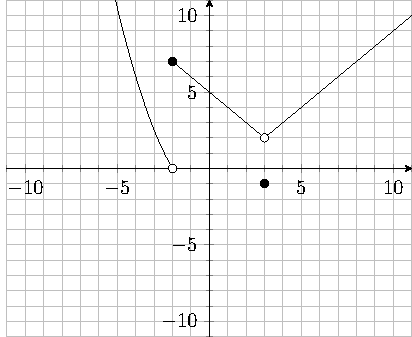
\includegraphics{finalgraph1.pdf}
\captionof{figure}{$f(x)$}\label{graph1exam1}%      only if needed  
\end{minipage}


\begin{questions}
\begin{multiplechoice}{5}
%8.5,8.6

\question According to the graph of $f(x)$, the $\lim_{x\to 3}f(x) $ equals which of the following.
\begin{answers}{3}
\ans $-3$
\ans $8$
\ans $-1$
\ans $2$
\ans The limit does not exist.
\end{answers}

%\textbf{Solution: d}


\question According to the graph of $f(x)$, the $\lim_{x\to -2^-}f(x) $ equals which of the following.
\begin{answers}{3}
\ans $7$
\ans $0$
\ans $-2$
\ans $-5$
\ans The limit does not exist.
\end{answers}

%\textbf{Solution: a}\\

\question According to the graph of $f(x)$, the $\lim_{x\to 5}f(x) $ equals which of the following.
\begin{answers}{3}
\ans $8$
\ans $4$
\ans $-1$
\ans $0$
\ans The limit does not exist.
\end{answers}

%\textbf{Solution: b}\\




\question According to the graph of $f(x)$, the function $f(x)$ is not continuous at $x=3$ because
\begin{answers}{3}
\ans there is a horizontal asymptote at $x=3$. 
\ans there is a vertical asymptote at $x=3$.
\ans $f(x)$ is not defined at $x=3$.
\ans $\lim_{x\to 3}f(x)$ does not exist.
\ans there is a removable discontinuity at $x=3$
\end{answers}

%\textbf{Solution: e}

%11.1,2

\newpage

\question The graph of $g(x)$ is given below.\\

\begin{minipage}{\linewidth}% to keep image and caption on one page
\centering
\makebox[\linewidth]{}
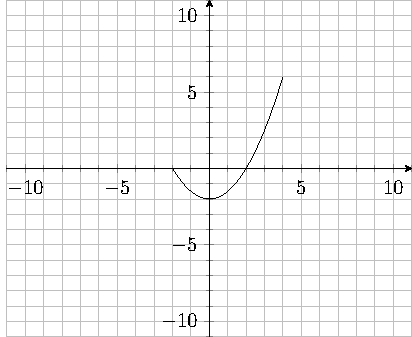
\includegraphics{exam1graph2.pdf}
\captionof{figure}{$g(x)$}\label{graph2exam1}%      only if needed  
\end{minipage}
According to the graph above, the domain and range of $g(x)$ are
\begin{answers}{2}
\ans Domain: $[-4,4]$, Range: $[-6,2]$
\ans Domain: $[-2,-6]$, Range: $[-2,4]$
\ans Domain: $[-4,4]$, Range: $[-4,2]$
\ans Domain: $[-6,2]$, Range: $[-2,4]$
\ans Domain: $[-2,4]$, Range: $[-2,6]$
\end{answers}
% Answer: 232/99

\question Find the domain of $f(x) = \frac{1}{x^2 - 16}$.
\begin{answers}{2}
\ans $(-2,2) \cup (2, \infty)$
\ans $(-\infty, -4) \cup (-4,4) \cup (4, \infty) $
\ans  $(-\infty, -4) \cup (0, \infty)$
\ans  $(-\infty, -2) \cup (-2,2) \cup (2, \infty)$
\ans $[-2,2)$
\end{answers}


\question Let $f(x) = \sqrt{4-x^2}$ and $g(x)=\ln(x)$.  What is the domain of $f(x)g(x)$?
\begin{answers}{2}
\ans $(0,2]$
\ans $[-1,2)$
\ans $[-2,\infty)$
\ans $(0,\infty)$
\ans $[-2,2]$
\end{answers}

\newpage

%(25 - x^2) - 16 / 3 - x
% 9 - x^2 / 3 -x
% 3 + x
% 6

\question Evaluate $\displaystyle \lim_{x \to 3} \frac{\sqrt{25-x^2} - 4}{3-x}$.
\begin{answers}{3}
\ans $1$
\ans $\frac{\sqrt{23} - 4}{2}$
\ans $-2$
\ans $\frac{3}{4}$
\ans $9$
\end{answers}



\question Given a function $f(x)$, then the graph of $2f\left(3 - x\right)$ will be
\begin{answers}{2}
\ans the graph of $f(x)$ shrunk horizontally by a factor of 2, shifted 4 units up, then reflected across the $x$-axis.
\ans the graph of $f(x)$ stretched vertically by a factor 3, shifted 2 units up, then reflected across the $y$-axis.
\ans the graph of $f(x)$ stretched vertically by a factor of 2, shifted 3 units to the right, then reflected across the $y$-axis.
\ans the graph of $f(x)$ stretched vertically by a factor of 2, shifted 3 units to the left, then reflected across the $y$-axis.
\ans the graph of $f(x)$ shrunk horizontally by a factor of 3, shifted 4 units to the right, then reflected across the $x$-axis.
\end{answers}



\question A bacteria population doubles every 47 minutes.  If the initial population is 1000 bacteria, how many bacteria will there be after 5 hours?
\begin{answers}{3}
\ans $4.2 \times 10^4$
\ans $3.2 \times 10^3$
\ans $4.3 \times 10^3$
\ans $1.2 \times 10^3$
\ans $8.3 \times 10^3$
\end{answers}


%% EXAM 2

\question Find the derivative of the function $f(x) = \frac{3}{x^3} - 4x^2 + 3$.
\begin{answers}{2}
\ans $-\frac{15}{x^2} - 8x$
\ans $-\frac{15}{x^2} + 3$
\ans $-\frac{9}{x^4} -8x$
\ans $-\frac{9}{x^4} - 4$
\ans $-\frac{10}{x} - 3$
\end{answers}

\newpage


For the next two questions, use the following graph of $f'(x)$:\\


\begin{minipage}{\linewidth}% to keep image and caption on one page
\centering
\makebox[\linewidth]{}
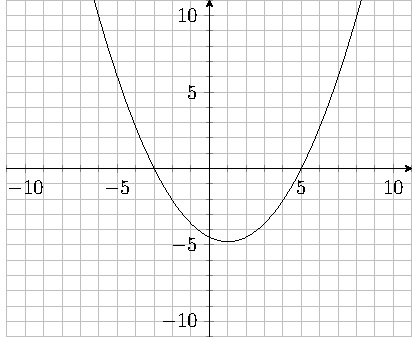
\includegraphics{finalgraph3.pdf}
\captionof{figure}{$f'(x)$}\label{graph1exam1}%      only if needed  
\end{minipage}


\question According to the graph of $f'(x)$, the original function $f(x)$ has a local maximum at
\begin{answers}{3}
\ans $-5$
\ans $-3$
\ans $0$
\ans $1$
\ans $5$
\end{answers}


\question According to the graph of $f'(x)$, the original function $f(x)$ is concave upward in which interval(s)?
\begin{answers}{2}
\ans $(-\infty, \infty)$
\ans $(-\infty, -3) \cup (1,5)$
\ans $(1, \infty)$
\ans $(-\infty, -3)$
\ans The original function $f(x)$ is never concave up.
\end{answers}



\question A vertical spring is released at time $t = 0$ seconds and begins to oscillate in a straight vertical line.
The height of its endpoint above the ground in meters is given by the function
$$h(t) = 3 - 0.2\cos(2t)$$
To two decimal places, what is the velocity (in meters/second) of the spring's endpoint at time $t = 3$ ?
\begin{answers}{3}
\ans -0.11
\ans -0.06
\ans 0.12
\ans 2.12
\ans 2.84
\end{answers}

\newpage

\question Find the linear approximation to $\sqrt{x^2+8}$ at $x = 1$
\begin{answers}{2}
\ans $3x + \sqrt{8}$
\ans $\frac{2}{3}x + 3$
\ans $\frac{1}{3} x + \frac{8}{3}$
\ans $x + \sqrt{8}$
\ans $\frac{1}{3} x + 3$
\end{answers}


\question We are given an unknown function $f(x)$ such that $f'(2) > 0$ and $f''(2) < 0$.
We can conclude that at $x = 2$, the function $f(x)$ has 
\begin{answers}{2}
\ans a local min.
\ans a local max.
\ans an inflection point.
\ans an undefined derivative.
\ans none of the above.
\end{answers}

\question Calculate the equation of the tangent line to $y = \frac{1}{x}$ at $x = 2$
\begin{answers}{2}
\ans $y = -\frac{1}{2}x + \frac{1}{2}$
\ans $y = -\frac{1}{2}x + 2$
\ans $y = -\frac{1}{4}x + \frac{1}{2}$
\ans $y = x + \frac{1}{2}$
\ans $y = -\frac{1}{4}x + 1$
\end{answers}





%% EXAM 3


\question Find the absolute maximum and minimum values for the function 
$f(x) = \ln(x^2 + 1)$ on the interval $[-1, 3]$
\begin{answers}{1}
\ans maximum value $= 2.30$, minimum value $ = 1.1$
\ans maximum value $= 3.62$, minimum value $ = 1.1$
\ans maximum value $= 2.30$, minimum value $ = 0$
\ans maximum value $= 3.62$, minimum value $ = 0$
\ans maximum value $= 1.32$, minimum value $ = 1$
\end{answers}

\newpage

\question Find the derivative of the function $f(x) = \tan(x e^x)$.
\begin{answers}{2}
\ans $(1+x)e^x \sec^2(xe^x) $
\ans $e^x \sec^2(xe^x) $
\ans $(1+x)e^x \tan(xe^x) $
\ans $e^x \cos^2(xe^x) $
\ans $\sec^2(xe^x) $
\end{answers}


\question If $f'(x) = \frac{1}{2\sqrt{x}}$ and $f(9) = 5$
\begin{answers}{2}
\ans $f(x) = \frac{3}{4}x^{-3/2} +  \frac{11}{4}$
\ans $f(x) = \sqrt{x} + \frac{7}{2}$
\ans $f(x) = \frac{1}{2}\sqrt{x} + 3$
\ans $f(x) = \frac{1}{2}\sqrt{x} + \frac{7}{2}$
\ans $f(x) = \sqrt{x} + 2$
\end{answers}


\question A particle moves along a wire with velocity $v(t) = 4\cos(2t)$.  Find the
net change in position between time $t = 0$ and $t = \pi$
\begin{answers}{2}
\ans $1  + \pi$
\ans $2\pi$
\ans $4\pi$
\ans $0$
\ans $\frac{\pi}{2}$
\end{answers}


% 600 = 2s^2 + 4sl
% V = s^2l
% 4sl = 600 -2s^2
% l = 600 -2 s^2 / 4 s
% V =  (600s - 2 s^3)/ 4
% V' = 150 - (3s^2/2)
% s = 10

\question Alex wants to make a box with a square base, closed on all sides.  He has 600 square inches of cardboard.  What is the maximum volume of the box in cubic inches?
\begin{answers}{3}
\ans $598.32$
\ans $643.60$
\ans $1000$
\ans $1284.81$
\ans $1500$
\end{answers}


\question Calculate the indefinite integral 
$\displaystyle \int \frac{1}{x} + \sec(3x) \tan(3x) \, dx$
\begin{answers}{2}
\ans $ \ln |x| + 3 \sec(3x) + C$
\ans $\frac{2}{x^2} + \frac{1}{3}\sec(3x) + C$
\ans $\ln|x|  + \frac{1}{3}\sec(3x) + C$
\ans $-\frac{2}{x^2}  + \frac{1}{3}\tan(3x) + C$
\ans $\ln |x| + \frac{1}{3}\cot(3x) + C$
\end{answers}


\newpage

\question Use the fundamental theorem of calculus to find the derivative of 
$\displaystyle f(x) = \int_1^{x^2} \sin(\cos(t)) \, dt$
\begin{answers}{2}
\ans $\sin(\cos(x^2))$
\ans $x^2 \sin(\cos(x^2))$
\ans $(x^2 - 1) \sin(\cos(x^2))$
\ans $2x \sin(\cos(x^2))$
\ans $(2x - 1) \sin(\cos(x)$
\end{answers}

\question Use the geometric shape of the graph to find the integral 
$\displaystyle \int_{-3}^2 f(x)$ where 
$$ f(x) = 
\begin{cases}
5, & x \le 0 \\
\sqrt{4 - x^2}, & x > 0
\end{cases}
$$
\begin{answers}{2}
\ans $2\pi$
\ans $\frac{15}{2} + \frac{1}{4}\pi$
\ans $15 + \pi$
\ans $15 + 2\pi$
\ans $10  + \frac{\pi}{2}$
\end{answers}

\question The acceleration of a particle is given by $a(t) = 6\sin(t)$.  The position
of the particle at time $t = 0$ is $s(0) = 3$.  The initial velocity of the particle is $v(0) = -7$.
The position function for the particle is
\begin{answers}{2}
\ans $s(t) = -3t^2 + 5t + 3$ 
\ans $s(t) = -6 \sin(t) -t + 3$
\ans $s(t) = -6 \cos(t) -t + 6$
\ans $s(t) = -6 \cos(t) - 13t + 3$
\ans $s(t) = -6 \sin(t) - 13t + 3$
\end{answers}

\question Calculate $\int_1^{e^3} \frac{(\ln(x))^2}{x} \, dx$.
\begin{answers}{2}
\ans $9$ 
\ans $\frac{1}{3} e^{3} - 1$
\ans $2e^{-3}$
\ans $\frac{1}{3}$
\ans $8$
\end{answers}

\question Calculate the area between the curves $y = x$ and $y = x^2$.
\begin{answers}{3}
\ans $\frac 1 3$ 
\ans $\frac 1 6$ 
\ans $\frac 2 3$ 
\ans $1$ 
\ans $- \frac 1 2$ 
\end{answers}

\question What is the average value of the function $f(x) = \sin(x)$ on $[0, \pi]$
\begin{answers}{3}
\ans $2$
\ans $-2\pi$
\ans $-\frac{\pi}{2}$
\ans $\pi$
\ans $\frac{2}{\pi}$
\end{answers}


% ln(y+2/(y-3)) = x - 7
% \frac{y+2}{y-3} = e^{x - 7}
% y +2 = (y - 3)e^{x-7}
% y(1 - e^{x-7}) = -3e^{x-7} - 2
% C
\question Find the inverse function to $f(x) = \ln(x+2) - \ln(x-3) + 7$.
\begin{answers}{2}
\ans $\frac{-2e^{x-7} - 3}{-e^{x-7} - 1}$
\ans $\frac{-3e^{x-7} - 2}{-e^{x-7} - 1}$
\ans $\frac{-3e^{x-7} - 2}{-e^{x-7} + 1}$
\ans $\frac{-2e^{x-1} - 3}{-e^{x-1} + 7}$
\ans $\frac{-2e^{x-3} - 2}{-e^{x-3} - 7}$
\end{answers}

\end{multiplechoice}
\end{questions}
\end{document}

*************************************************************************
*************************************************************************
